\section{数据科学导论部分}\label{SecDataScience}
\begin{center}
    Instructor: Sheng Yu
\end{center}

    This section contains basic data acquisition, data cleaning, data processing, date visualization methods. Details for data analysis are not covered.

\begin{point}
    Road to Data Scientist
\end{point}

\begin{figure}[H]
    \centering
    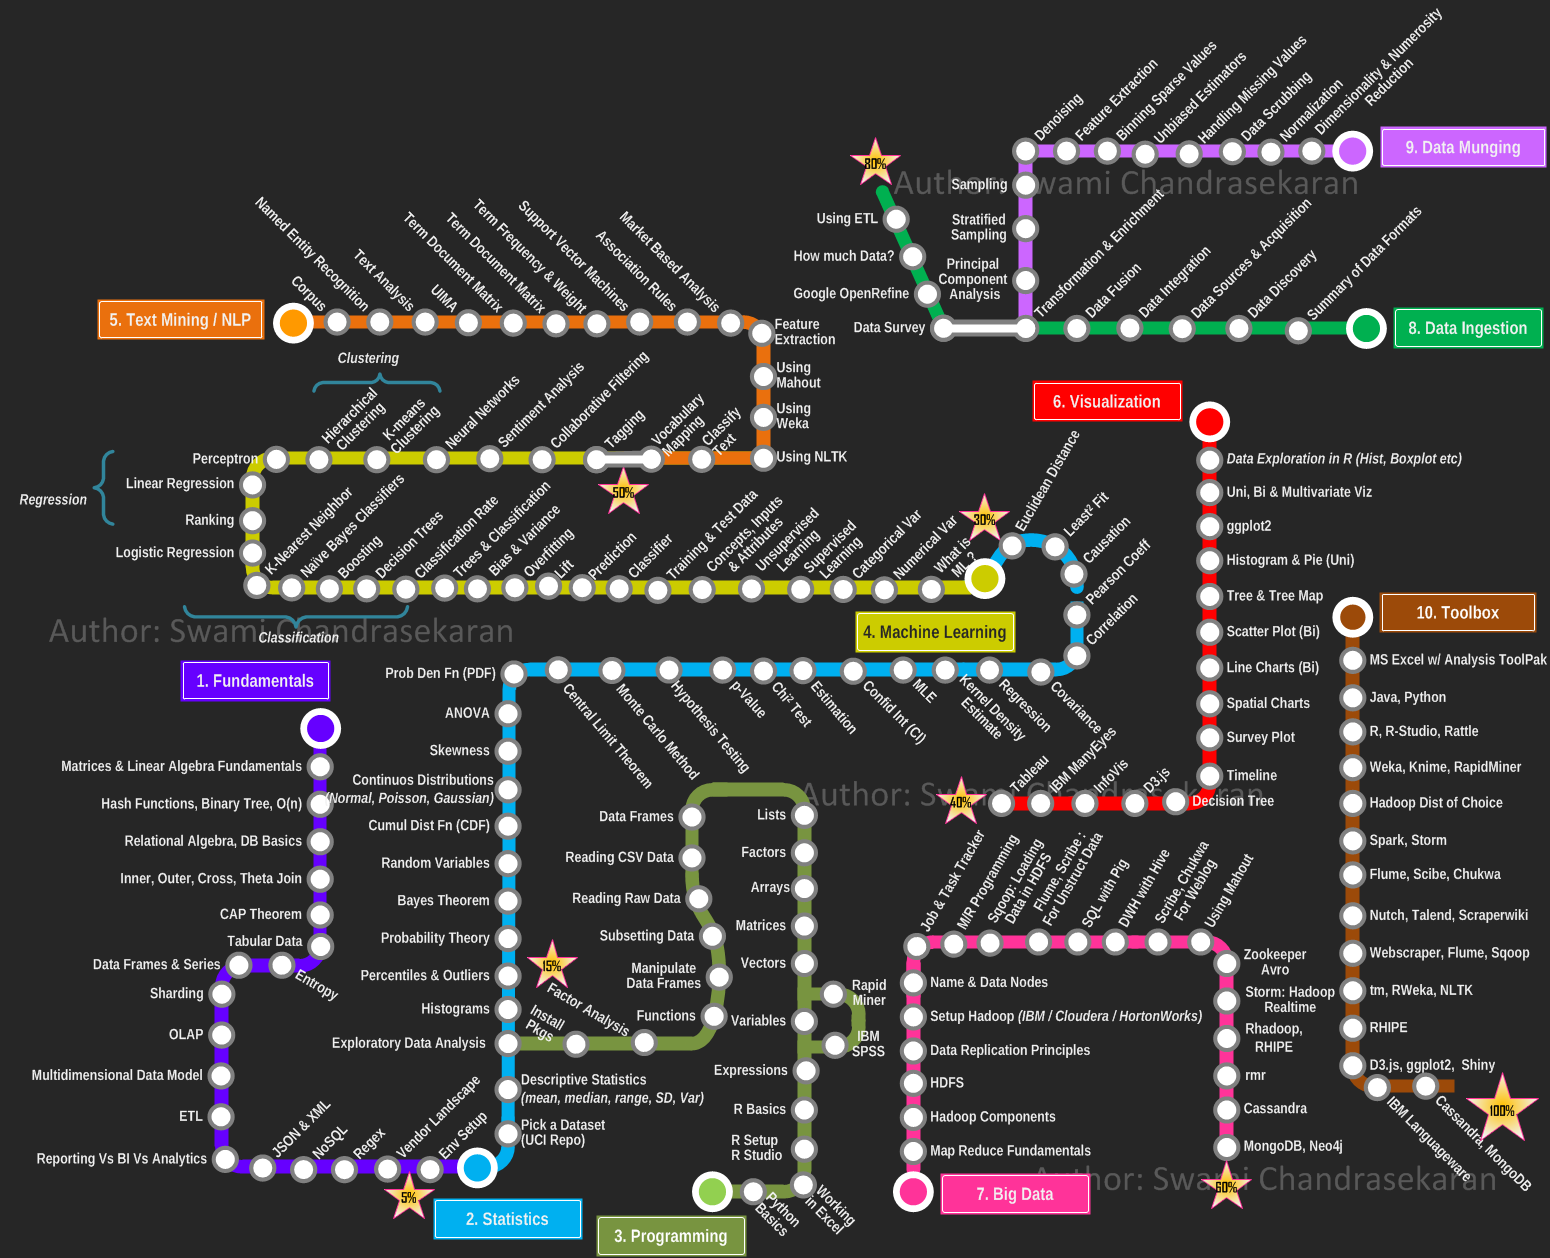
\includegraphics[width=\linewidth]{sections/images/RoadToDataScientist1.png}
    \caption{Road to Data Scientist}
    \label{RoadToDataScience}
\end{figure}


Comparison of \lstinline|R|, \lstinline|python|:focus on different aspects of `Statistics':
\begin{itemize}[topsep=2pt,itemsep=0pt]
    \item Differnece in programming philosophy: \lstinline|R| for data analysis and \lstinline|python| for data processing
    \item Difference in operating domain: \lstinline|R| for statistical programming while \lstinline|python| for general programming.
\end{itemize}



\subsection{Basic R. Manipulation}


\subsubsection{Installation and Maintenance of R.}
\begin{point}
    \textbf{Installing and Updating} 
\end{point}

\noindent  \lstinline|R.|: update by delete old version and install new version.
\begin{itemize}[topsep=2pt,itemsep=0pt]
    \item In CRAN (The Comprehensive \lstinline|R| Archive Network):\index{CRAN (The Comprehensive R Archive Network)} \url{https://cran.r-project.org}
    \item In Mirror@TUNA: \url{https://mirrors.tuna.tsinghua.edu.cn/CRAN}
\end{itemize}

\noindent RStudio: \url{https://www.rstudio.com}


\begin{point}
    \textbf{Running}  \lstinline|R.| \textbf{command} :
\end{point}

\begin{itemize}[topsep=2pt,itemsep=0pt]
    \item In \lstinline|R.| GUI\index{GUI (Graphical User Interface)};
    \item In \lstinline|R.| command line terminal;
    \item \lstinline|R. CMD BATCH|;
    \item \lstinline|Rscript|;
        \begin{itemize}[topsep=2pt,itemsep=0pt]
        \item Use \lstinline|>| to redirect output(overwrite);
        \item Use \lstinline|>>| to append output.
        \end{itemize}
\end{itemize}



\begin{point}
    \lstinline|R.| \textbf{package library}: packages are collection of \lstinline|R.| functions (as well as test data and sample code).
\end{point}

\begin{itemize}[topsep=2pt,itemsep=0pt]
    \item \lstinline|.libPaths()| show package library location\footnote{Unlike in \lstinline|C| or \lstinline|python| where \lstinline|.| is an operator, \lstinline|.| in \lstinline|R.| is just a common character, without special meaning.
    
    This feature can be used in naming self-defined functions: use \lstinline|.FUN_NAME1| for within-project function while \lstinline|FUN_NAME2| for external interface.} ;
    \item \lstinline|library('PACKAGE_NAME1','PACKAGE_NAME2',...)| load packages.
    \item \lstinline|install.packages('PACKAGE_NAME1','PACKAGE_NAME2',...)| install package from CRAN/mirrors;
    \item \lstinline|installed.packages()| show all installed packages;
    \item \lstinline|updata.packages(checkBuilt = TRUE, ask = FALSE)| update installed packages;
\end{itemize}

\begin{point}
    \textbf{Working directory}  manipulation:
\end{point}

\begin{itemize}[topsep=2pt,itemsep=0pt]
    \item \lstinline|getwd()| get current working directory;
    \item \lstinline|setwd('TARGET_PATH')| set working directory (as an existing path).
    \item \lstinline|dir()| show current directory.
\end{itemize}

\begin{point}
    Recommended \lstinline|R.| \textbf{Project Organization} : working directory organized like
\end{point}

\begin{itemize}[topsep=2pt,itemsep=0pt]
    \item \lstinline|data/| folder for structured original dataset;
    \item \lstinline|result/| folder for output result;
    \item \lstinline|presentation/| folder for result representing slides/reports/etc.;
    \item \lstinline|.r| project file $ \times n $.
\end{itemize}

\begin{point}
    Looking for \textbf{Help/Example}  of function:
\end{point}

\begin{itemize}[topsep=2pt,itemsep=0pt]
    \item \lstinline|?FUN_NAME()|;
    \item \lstinline|help('FUN_NAME')|;
\end{itemize}

\subsubsection{Data Structure and Basic Manipulation in R.}

\begin{point}
    Atomic Classes
\end{point}
\begin{itemize}[topsep=2pt,itemsep=0pt]
    \item \lstinline|'abc'| Character;
    \item \lstinline|3L| Integer;
    \item \lstinline|2.4| Numeric;
    \item \lstinline|TRUE,FALSE,T,F| Logical;
    \item Special types: \lstinline|NA|, \lstinline|NaN|, \lstinline|NULL|, \lstinline|Inf|
\end{itemize}

\begin{point}
    Operators
\end{point}
\begin{itemize}[topsep=2pt,itemsep=0pt]
    \item Numerical Operators: \lstinline|+|, \lstinline|-|, \lstinline|*|(multiply by column), \lstinline|/|, \lstinline|%*%|(matrix multiply), \lstinline|^|, \lstinline|%%|(remainder operate);
    \item Logical Operators: \lstinline|==|,etc.; \lstinline|&| and \lstinline{|} for common operator, \lstinline|&&| and \lstinline{||} for comparing the first element;
    \item Round a numeric:
    \begin{itemize}[topsep=2pt,itemsep=0pt]
        \item \lstinline|as.integer()|, round towards 0
        \item \lstinline|trunc()|
        \item \lstinline|ceiling()|
        \item \lstinline|floor()|
        \item \lstinline|round(NUMBER_TO_ROUND,digits = DIGITS)|
    \end{itemize}
\end{itemize}

\begin{point}
    Type Conversion
\end{point}

\begin{itemize}[topsep=2pt,itemsep=0pt]
    \item First need to meet the need of 
\end{itemize}

    
    Key Criterion: when converting mixed type in to the same type, use the type with more compatibility.
\begin{itemize}[topsep=2pt,itemsep=0pt]
    \item Logical $ \to $ Numeric: 
\end{itemize}

    

\begin{point}
    Data Structure
\end{point}
\begin{itemize}[topsep=2pt,itemsep=0pt]
    \item \textbf{Atomic Vector} : Column vector is the \textbf{basic} data structure in \lstinline|R.| (scalar is length=1 vector).
    
    Only data of the same class can be held in one vector.
    
    Initialization:
    \begin{itemize}[topsep=2pt,itemsep=0pt]
        \item Ordinary way: 
        \begin{itemize}[topsep=2pt,itemsep=0pt]
            \item \lstinline|c(1,2,3)|, \lstinline|c(T,FALSE,TRUE)|, \lstinline|c('a',NA,'b')|
            \item \lstinline|vector(mode = MODE,length = LENGTH)|
            \item \lstinline|logical(LENGTH)| return \lstinline|FALSE| vector 
        \end{itemize}
        
        where \lstinline|c()| for `combine'; 
        
        \lstinline|c()| combines all things into one vector, e.g. \lstinline|c(c(1,2,3),c(1,2))=c(1,2,3,4,5)|.
        \item Sequence vector: 
        \begin{itemize}[topsep=2pt,itemsep=0pt]
            \item \lstinline|1:3.5=c(1,2,3)|, \lstinline|3:1=c(3,2,1)|
            \item \lstinline|seq(from, to ,by, length.out)|, \lstinline|length.out| for total vector length;
            \item \lstinline|rep(SEQ_TO_REP, times, lenght.out ,each)|, used in $ k $-fold cross validation labelling.
        \end{itemize}
    \end{itemize}
    
    Operations:
    \begin{itemize}[topsep=2pt,itemsep=0pt]
        \item between vectors of different length \lstinline|SHORT| and \lstinline|LONG|: First \lstinline|SHORT <- rep(SHORT,|\\\lstinline| length.out=length(LONG))|. Then operate \lstinline|SHORT| and \lstinline|LONG|.
        \item Element access: \lstinline|a[i]|
    \end{itemize}
    
         
    \fbox{
        \begin{minipage}{0.9\linewidth}

    \textbf{Vectorized Operation}: All operation in \lstinline|R.| are based on vector, and vectorized operation is Parallel Arithmetic, which is \textbf{much faster} than loop such as \lstinline|for| $ \longrightarrow $ Consider using vectorized opertion when writing code for \textbf{Speed}! Detail see \autoref{SubSubSectionVectorizedOperation}.
        \end{minipage}
    }

    \item \textbf{Factor} : A special kind of `vector' in \lstinline|R.|, used to label discrete categorical data.\footnote{Factor vector is stored as integer vector.}
    
    Initialization:

    \lstinline|factor(FACTOR_SEQ, levels = FACTOR_LEVEL, labels = ...)|, \lstinline|FACTOR_LEVEL| is the `rank' of each factor, \lstinline|labels| is the `tag' of levels. 

    A quick way to factorize a numeric vector \lstinline|x| by interval division:
    
    \lstinline|cut_number(x, NUM_OF_LEVELS)|

    \item \textbf{Matrix} : Only data of the same class can be held in one matrix.
    
    Initilaization:
    
    \lstinline|matrix(DATA_SEQ, nrow, ncol, byrow = FALSE, dimnames = NULL)|
    
    If \lstinline|length(DATA_SEQ) < nrow*ncol|, then \lstinline|DATA_SEQ| is repeated with \lstinline|length.out=nrow*ncol|. 
    
    Default: fill by column (because matrix is stored by column).

    Operation:
    \begin{itemize}[topsep=2pt,itemsep=0pt]
        \item Common operators \lstinline|+-*/^| etc. operate in column-by-column mode (vectorized operation).
        \item Binding matrix: \lstinline|cbind| for \lstinline|[A,B]| and \lstinline|rbind| for \lstinline|[A;B]|
        \item Transpose: \lstinline|t()|
        \item Matrix multiplication: \lstinline|%*%|
        \item Inverse matrix: \lstinline|solve()| (The essence of inversion is solving linear equations)
        \item Diagonal matrix:
        \begin{itemize}[topsep=2pt,itemsep=0pt]
            \item \lstinline|diag(VECTOR)| returns a matrix $ \mathrm{diag}\{ $\lstinline|VECTOR|$ \} $
            \item \lstinline|diag(MATRIX)| returns the diagonal element vector
        \end{itemize}
        \item Element access: \lstinline|a[i,j]|, \lstinline|a$OBJECT_NAME|
        \item Dimension: \lstinline|dim()|, \lstinline|nrow()|, \lstinline|ncol()|
        \item Rank: \lstinline|qr(MATRIX)$rank|
        % \item 
    \end{itemize}
    
    \item \textbf{List} : A pack containing various datatype, generally also a kind of vector(but not atomic vector)
    
    Initialization: \lstinline|list(OBJECT1,OBJECT2,...)|

    Element access: \lstinline|a[[i]]|
    \item \lstinline|data.frame|: `Mixture' of matrix and list. \lstinline|data.frame| is actually a kind of list(with some constraint), organized in the shape of matrix (but allowing different datatype for different columns, each column is a list object).
    
    Each column of \lstinline|data.frame| has name: \lstinline|names(DATA_FRAME)|, \lstinline|colnames(DATA_FRAME)|

    Element access: \lstinline|a[i,j]|, \lstinline|a[[i]]|, \lstinline|a$COL_NAME|
\end{itemize}

    
\begin{point}
    Data Read \& Write
\end{point}
\begin{itemize}[topsep=2pt,itemsep=0pt]
    \item Common R\&W: \lstinline|read.|/\lstinline|write.|
    \begin{itemize}[topsep=2pt,itemsep=0pt]
        \item \lstinline|read.table(FILE_NAME,header = FALSE,sep,colClasses,stringAsFactors = FALSE)|
        \item[${\color{red}\star }$] \lstinline|read.csv()| basically the same as \lstinline|read.table|
        \item[${\color{red}\star }$] \lstinline|write.table(DF,FILE_NAME,sep,row.names=FALSE)|
        \item \lstinline|readxl::read_xlsx(FILE_NAME,sheet = SHEET_NUM,range = 'RANGE')|
    \end{itemize}

    Some relative arguments:
    \begin{itemize}[topsep=2pt,itemsep=0pt]
        \item \lstinline|quote="'"|, use \lstinline|'| to quote/identify string, set \lstinline|quote=''| to avoid misread strings such as `Levene's Test'
        \item \lstinline|encoding='UTF-8'|, char encoding system, used especially for dataset containing CJK char.
        \item \lstinline|nrows=LINE_NUM| read first \lstinline|LINE_NUM| lines
        % \item 
    \end{itemize}

    \item Large Data Read \& Write: 
    \begin{itemize}[topsep=2pt,itemsep=0pt]
        \item preset \lstinline|colClasses|
        
\begin{lstlisting}[language=R]
temp.dat <- read.table(FILE_NAME, nrows = 100)
classes <- sapply(temp.dat, class)
dat <- read.table(FILE_NAME, colClasses = classes)
\end{lstlisting}
        \item \lstinline|readr::read_delim(FILE_NAME,delim=SEP)| can speed up
    \end{itemize}
    
    \item Text Write: \lstinline|sink(FILE_NAME,append=FALSE)|, write output into a file, the same as \lstinline|>| in terminal.
    \item \lstinline|.RData| Binary Format Read \& Write: RW in \lstinline|.RData| format, fast to load.
    \begin{itemize}[topsep=2pt,itemsep=0pt]
        \item \lstinline|save(DF,file = FILENAME)|
        \item \lstinline|load(FILE_NAME)|
    \end{itemize}
\end{itemize}

    




\subsubsection{Functions and Control Flow}
\begin{point}
    Program Speed:
\end{point}

\lstinline|system.time({COMMAND})|

\begin{point}
    Function Call
\end{point}
\begin{itemize}[topsep=2pt,itemsep=0pt]
    \item \lstinline|FUN_NAME(ARGUs)|
    \item \lstinline|do.call('FUN_NAME',LIST_OF_ARGUs)|, look for a function naming \lstinline|FUN_NAME| in \lstinline|R.| and call. 
    \item \lstinline|a % NEW_OPRTR % b| to call self-defined binary operator.
    \item \lstinline|'*'| etc. used in \lstinline|apply(FUN = '*')|
    \item \lstinline|R.| allows auto-completion to \lstinline|ARGUs|, e.g. \lstinline|rep(0,length.out=10)| = \lstinline|rep(0,length=0)|
\end{itemize}


\begin{point}
    Function Definition
\end{point}

\begin{rcode}
    Basic function definition in \lstinline|R.|
\begin{lstlisting}[language=R]
FUNC_NAME <- function(ARG1 = ARG1_DEF_VALUE , ARG2, ...) {
    FUNCTION_BODY
}
\end{lstlisting}
\end{rcode}

More key elements in \lstinline|funtion{}|
\begin{itemize}[topsep=2pt,itemsep=0pt]
    \item \lstinline|return(RETURN_OBJ)| at the end of function, without \lstinline|return()|, output the last line
    \item \lstinline|stopifnot(COND1,COND2,...)| at the beginning of function, used to test \lstinline|ARG| class
    \item \lstinline|stop(ERROR_MESG)| output error message
    \item \lstinline|...| as a special argument
    \begin{itemize}[topsep=2pt,itemsep=0pt]
        \item Pass \lstinline|...| to another func in this function
        \item Handle arbitrary number of input
    \end{itemize}
    \item Function can be defined within function
    \item Function is a kind of variable $ \longrightarrow $ used in \lstinline|apply|, \lstinline|sapply| etc. for vectorized programming.
    \item Anonymous function: used in \lstinline|sapply(X,FUN=function(){STATs})| for quick definition
    \item \lstinline|FUNC_NAME| can be used for new-defined binary operator as \lstinline|'%NEW_OPRTR%' <- function()|
\end{itemize}


\begin{point}
    Flow Control
\end{point}

\begin{itemize}[topsep=2pt,itemsep=0pt]
    \item \lstinline|if| and \lstinline|else if|, example:
\begin{lstlisting}[language=R]
if(COND1) {
    STATEMENT
} else if(COND2) {
    STATEMENT
} else {
    STATEMENT
}
\end{lstlisting}
    \item \lstinline|ifelse(COND,IF_YES_STAT,IF_NO_STAT)| a vectorized version of \lstinline|for+if else|.

    \item \lstinline|for|: Loop in \lstinline|R.| is \textbf{Extremely Slow}, avoid loop, use \textbf{vectorized operation}.  
\begin{lstlisting}[language=R]
for(VAR in SEQ) {
    STATEMENT
}
\end{lstlisting}
    \item \lstinline|switch(TEST_EXPR,CASE1 = RETN1,CASE2 = RETN2,...)|
 
    
        
    

\end{itemize}







\subsubsection{Vectorized Operation}\label{SubSubSectionVectorizedOperation}
\begin{itemize}[topsep=2pt,itemsep=0pt]
    \item \lstinline|apply()| function series:
\begin{itemize}[topsep=2pt,itemsep=0pt]
    \item \lstinline|apply(MAT,MARGIN,FUN)| for matrix apply, \lstinline|MARGIN=1| for each row, \lstinline|2| for each column
    \item \lstinline|lapply(LIST,FUN)| for list/\lstinline|data.frame|, apply \lstinline|FUN| on each list elements,\lstinline|list| returned
    \item[$ \color{red}\star $] \lstinline|sapply(X,FUN)| for list/\lstinline|data.frame| apply+simplify, \lstinline|vector/matrix/list| returned
    \item \lstinline|tapply(X,INDEX,FUN)|: for each index, use \lstinline|FUN| respectively.
    \item \lstinline|mapply(FUN,ARGU_OF_FUN)|, use argument name to label \lstinline|ARGU_OF_FUN|, or causes bad readability. 
    
    Example:
\begin{lstlisting}[language=R]
mapply(function(x,y,z,k){(x+k)^(y+z)} , x = ,y = ,z = ,k = )
\end{lstlisting}
    \end{itemize}

    \item \lstinline|Vfunc <- Vectorize(FUNC_NAME)|: define vectorize version of function.
    \item \lstinline|with()| and \lstinline|within()|:
    \begin{itemize}[topsep=2pt,itemsep=0pt]
         \item \lstinline|with(DF,aggregate(PART,by,FUN))|
        \item \lstinline|with(DF,STATE),within(DF,STATE)|,
     \lstinline|within| allows new column append
    \end{itemize}
    \item \lstinline|outer(VEC1,VEC2,FUN)|: A Two-variate extension of \lstinline|mapply()|, output wedge of two vectors.
    \item \lstinline|ifelse(COND,YES_STAT,NO_STAT)|, vectorization supported.
\end{itemize}





\subsubsection{Subsetting}
\begin{itemize}[topsep=2pt,itemsep=0pt]
    \item By position: \lstinline|x[RANGE]|
    \begin{itemize}[topsep=2pt,itemsep=0pt]
        \item \lstinline|x[4]|
        \item \lstinline|x[-4]|: without the $ 4^\mathrm{th} $ item (different from \lstinline|python|, where selects reciprocal $ \mathrm{4^{th}}  $ element).
        \item \lstinline|x[2:4]|
        \item \lstinline|x[c(1,2,5)]|
    \end{itemize}
    \item By name: \lstinline|x[,'COL_NAMEs']|, \lstinline|x[,'COL_NAME1':'COL_NAME2']|
    \item By condition: basically, \lstinline|x[LOGI_VEC]|
    \begin{itemize}[topsep=2pt,itemsep=0pt]
        \item \lstinline|x[x==10]|
        \item \lstinline|x[x %in% c(1,3,4)]|, linear search, not based on hash algorithm\footnote{If really needed, use \lstinline|env()| to reset environment.}.
    \end{itemize}

    Usually used for conditional selection of \lstinline|data.frame|
    \item Subsetting for \lstinline|data.frame| and list: \lstinline|x[[RANGE]]|


    Simplified/Preserved subsetting: whether preserved datatype, e.g. df $ \to $ df (preserved) v.s. df $ \to $ vector (simplified).
\begin{table}[H]
    \centering
    \renewcommand\arraystretch{1.15}
    \begin{tabular}{lll}
        \hline
        DataType&Simplified&Preserved\\
        \hline
        vector&\multicolumn{2}{c}{\lstinline|x[[1]]]| / \lstinline|x[1]|}\\
        list&\lstinline|x[[1]]|&\lstinline|x[1]|\\
        factor&\lstinline|x[1:4,drop=T]|&\lstinline|x[1:4]|\\
        matrix&\lstinline|x[,1]|&\lstinline|x[,1,drop=F]|\\
        \lstinline|data.frame|&\lstinline|x[,1]|,\lstinline|x[[1]]|&\lstinline|x[,1,drop=F]|,\lstinline|x[1]|\\
        \hline
    \end{tabular}
    \caption{Simplified/Preserved subsetting}
\end{table}
    \item Other subsetting:
    \begin{itemize}[topsep=2pt,itemsep=0pt]
        \item \lstinline|%in%| 
        \item \lstinline|unique()|, return with each element appears only one times
        \item \lstinline|duplicated()|, \lstinline|TRUE| when appear the $ n>1 $ times
        \item \lstinline|which(x==4)|, return position of matched element
        \item \lstinline|which.min()|, \lstinline|which.max|, \lstinline|min()|, \lstinline|max()|
        \item \lstinline|grep(REGEX,X,value)|, search for elements with \lstinline|REGEX| pattern: \lstinline|value=F| returns position, \lstinline|value=T| returns elements, \lstinline|grepl(REGEX,X)| returns logical vector
        \item \lstinline|match(TO_BE_MATCHED,TARGET)|, returns the index of elements of \lstinline|TO_BE_MATCHED| in \lstinline|TARGET|
        
        \begin{rcode}
            Example:
\begin{lstlisting}[language=R]
vec1 <- c('a','a','b','b','d','d','b')
vec2 <- c('d','a','b')
match(vec1,vec2)
> [1] 2 2 3 3 1 1 3
\end{lstlisting}
        \end{rcode}
        \item \lstinline|subset(X,...)|, \lstinline|...| a series of select criterion. \textbf{not} allowed: \lstinline|subset(X,...) <- | 
    \end{itemize}
    \item Use subsetting to sample: \lstinline|DATA[sample(1:nrow(DATA),NUM_OF_SAMPLE,replace),]|, \lstinline|replace=T| for with replacement
\end{itemize}

\subsubsection{Data Manipulation With dplyr. And tidyr.}
    \lstinline|dplyr| and \lstinline|tidyr| are two useful package for data cleaning \& manipulation. Use package \lstinline|tidyverse| include both of them.

    \lstinline|tidyverse| for \lstinline|tidy|uni\lstinline|verse|, includes \lstinline|dplyr|, \lstinline|tidyr|, \lstinline|readr|, \lstinline|ggplot2|, \lstinline|stringr|, etc.

\begin{point}
    \lstinline|%>%| pipe in \lstinline|tidyverse|: functions in \lstinline|tidyverse| use \lstinline|FUNC(DF,...)|, where \lstinline|DF| can be passed on by \lstinline|%>%|.

\end{point}


\begin{point}
    \lstinline|dplyr| Package. 
\end{point}

\begin{itemize}[topsep=2pt,itemsep=0pt]
    \item Cheet Sheet: \url{https://nyu-cdsc.github.io/learningr/assets/data-transformation.pdf}
    \item \lstinline|select(DF,...)|, where \lstinline|...| can use column index/name range as in subsetting, or some helper function for advanced subsetting:
    \begin{itemize}[topsep=2pt,itemsep=0pt]
        \item matching position:
        \begin{itemize}[topsep=2pt,itemsep=0pt]
            \item \lstinline|everything()|
            \item \lstinline|last_col()|
        \end{itemize}
        \item matching column name:
        \begin{itemize}[topsep=2pt,itemsep=0pt]
            \item \lstinline|start_with('PATTERN')|, \lstinline|end_with('PATTERN')|, \lstinline|contains('PATTERN')|
            \item \lstinline|match('REGEX')|, column name with \lstinline|REGEX| pattern
            \item \lstinline|num_range('x',1:4)| delect column name \lstinline|c('x1','x2','x3','x4')|
            \item \lstinline|any_of(CHR_VEC)| select column from \lstinline|CHR_VEC|
        \end{itemize}
        \item \lstinline|where(FUN)|, select those \lstinline|FUN(COL_NAME)| returns \lstinline|TRUE|
    \end{itemize}
    \item \lstinline|filter(DATA,CONDs)|, select elements with \lstinline|CONDs| conditions
    \item \lstinline|arrange(DATA,COL)|, sort by \lstinline|COL|, \lstinline|arrange(DATA,desc(COL))| for descending order
    \item \lstinline|mutate(DATA,...)|, append new columns according to \lstinline|...| definition; \lstinline|transmute()| drops original columns.
    
    \lstinline|...| definition can use advanced window function:
    \begin{itemize}[topsep=2pt,itemsep=0pt]
        \item \lstinline|lead(COL)|,\lstinline|lag(COL)|, e.g. \lstinline|lead(COL)[i]|=\lstinline|COL[i+1]|, can use \lstinline|...=COL-lead(COL)| for differnetial
        \item \lstinline|dense_rank(COL)|, \lstinline|percent_rank(COL)| rank number
        \item \lstinline|ntile(COL,N)| break into \lstinline|N| groups labeling \lstinline|1:N|
        \item \lstinline|cume_dist(COL)|, \lstinline|cummean(COL)|, \lstinline|cumsum(COL)|, \lstinline|cummax(COL)|, \lstinline|cummin(COL)|, etc. cumulative value
    \end{itemize}
    
    \item \lstinline|summarise(data,...)|, \lstinline|...| for summarise function.

    \item Row selection:
    \begin{itemize}[topsep=2pt,itemsep=0pt]
        \item \lstinline|slice(DF,ROW_RANGE)|
        \item \lstinline|distinct(DF)| remove duplicated rows
        \item \lstinline|sample_frac(DF,FRAC,replace)|, sample \lstinline|FRAC| fraction from \lstinline|DF|
        \item \lstinline|sample_n(DF,N,replace)|, sample \lstinline|N| cases from \lstinline|DF|
        \item \lstinline|top_n(DF,AMOUNT,RANK_COL)| select \lstinline|AMOUNT| top ranking by \lstinline|RANK_COL| cases
    \end{itemize}
    \item Data combining see slides.
\end{itemize}

\begin{point}
    \lstinline|tidyr| Package
\end{point}
\begin{itemize}[topsep=2pt,itemsep=0pt]
    \item Cheet Sheet: \url{https://leadousset.github.io/intro-to-R/cheatsheet_tidy.pdf}
    \item \lstinline|gather(DF,key='KEY_NAME',value='VALUE_NAME',...,na.rm)|, melt a \lstinline|data.frame|. 
    
    e.g. \lstinline|gather(df,'KEY','VALUE',c('COL1','COL2','COL3'))| transfers \lstinline|...| as:
    \[
        \begin{matrix}
            \text{ID}&\text{COL1}&\text{COL2}&\text{COL3}\\
            1&a_1&b_1&c_1\\
            2&a_2&b_2&c_2\\
            \vdots&\vdots&\vdots&\vdots
        \end{matrix}
        \quad\to\quad
        \begin{matrix}
            \text{ID}&\text{KEY}&\text{VALUE}\\
            1&\text{COL1}&a_1\\
            2&\text{COL1}&a_2\\
            \vdots&\vdots&\vdots\\
            1&\text{COL2}&b_1\\
            2&\text{COL2}&b_2\\
            \vdots&\vdots\\
            1&\text{COL3}&c_1\\
            2&\text{COL3}&c_2\\
            \vdots&\vdots
        \end{matrix}
    \]
    \item \lstinline|spread(DF,key='KEY_NAME',value='VALUE_NAME')|, inverse of \lstinline|gather()|
    \item \lstinline|separate(DF,COL,into=SET_VEC,sep='REGEX')|, separate \lstinline|COL| into columns with name in \lstinline|SET_VEC|, sep according to \lstinline|sep|
    \item \lstinline|unite(DF,COL,SET_VEC,sep='')| inverse of \lstinline|separate()|
\end{itemize}

    


\subsection{Text Processing \& Text Mining}
    \begin{itemize}[topsep=2pt,itemsep=0pt]
        \item Data cleaning
        \item Data manipulation
        \item Information extraction: mode identifying/relation extraction
        \item Text mining: anaylzing token distribution, ignore word order
        \item NLP: concept identifying based on sentence; untimate goal: `understand' sentence meaning.
    \end{itemize}
    
    Tools for Text processing:
\begin{itemize}[topsep=2pt,itemsep=0pt]
    \item \lstinline|R.|: suitable for easy task 
    \item \lstinline|python.|: best
    \item \lstinline|java|: strong, but not suitable for deep learning
    \item \lstinline|c++|: fast, inadequate package
    \item \lstinline|Notepad++|/\lstinline|Vim|
\end{itemize}

    
        



\subsubsection{Basic Text Manipulation With stringr.}
\begin{point}
    \lstinline|R. base| \& \lstinline|stringr| package:
\end{point}

    The prior one is used more often

\begin{itemize}[topsep=2pt,itemsep=0pt]
    \item Cheet Sheet: \url{http://edrub.in/CheatSheets/cheatSheetStringr.pdf}
    \item \lstinline|str_length(STRING)|, \lstinline|nchar(STRING)|
    \item \lstinline|paste(...,collapse=NULL)|,\lstinline|str_c(...)|, both are vectorized operation
    
    Argument:
    \begin{itemize}[topsep=2pt,itemsep=0pt]
        \item \lstinline|sep|: sep between each \lstinline|...| corresponding elements, with \lstinline|collapse=NULL|, return a char vector
        \item \lstinline|collapse|: sep when combining \lstinline|collapse=NULL| vector elements, \lstinline|NULL| for not combining
        \item Special character: \lstinline|\t| tab, \lstinline|\r| \& \lstinline|\n| \& \lstinline|\r\n| new line, \lstinline|\xad| `-' at end on line for word-connecting
    \end{itemize}
    
    \item \lstinline|str_split(STRING,pattern='REGEX')|/\lstinline|strsplit()|, split string at \lstinline|REGEX| pattern fitted, list returned
    \item \lstinline|str_sub(STRING,start,end)|, \lstinline|substr()|. The \lstinline|start| char to \lstinline|end| char of string, use negative index as in \lstinline|python|.
     
    Can be used to replace: \lstinline|str_sub(...) <- REP_STR|
    \item \lstinline|str_locate_all('STRING',pattern='REGEX')|/\lstinline|str_match_all('STRING',pattern='REGEX')|

    \lstinline|grep(pattern='REGEX',x='STRING',value=T)|, search for elements with \lstinline|REGEX| pattern: \lstinline|str_locate_all()| or \lstinline|value=F|  returns position, \lstinline|str_match_all()| or \lstinline|value=T| returns elements.
    
    \item \lstinline|str_replace_all('STRING',pattern='REGEX',replacement='REP')|
    \lstinline|grepl(REGEX,X)| returns logical vector, include or not.
    \lstinline|str_extract_all('STRING',pattern='REGEX')|
    \item \lstinline|gsub(pattern='REGEX',replacement='REP',x='STRING')|, replace \lstinline|REGEX| field with \lstinline|REP|
    % \item Extracting word: 
    \item \lstinline|str_trim(...,side = )|, trim extra white space at \lstinline|side='both'|/\lstinline|'left'|/\lstinline|'right'|
    % \item Padding: \lstinline|str_pad()| append space
\end{itemize}




\subsubsection{Regular Expression}
    Regular expression is a text pattern/mode. abbr. regex/regexp. Regex is supported in most common language, same syntax used.

    Tutorial: \url{https://www.runoob.com/regexp/regexp-tutorial.html}

\begin{point}
    Key Elements
\end{point}

\begin{itemize}[topsep=2pt,itemsep=0pt]
    \item Literal: common char, e.g. \lstinline|a|. Include most char on keyboard. Upper/Lower case sensitive.
    \item Metacharacters: \lstinline!\^$.|?*+()[]{}!, use e.g. \lstinline|\.| to escape meaning.
    
    Note: when typing regex in programming language, sometimes use \lstinline|\\.|: \lstinline|\\.| $ \xrightarrow[]{\text{language interpreter}}  $ \lstinline|\.| $ \xrightarrow[]{\text{regex interpreter}}  $ identifying \lstinline|.|

    \item Character Class: \lstinline|[]|, identify one of elements in \lstinline|[]|. \lstinline|^| within \lstinline|[]| for $ \complement $. 
    \begin{itemize}[topsep=2pt,itemsep=0pt]
        \item e.g. \lstinline|gr[ae]y| identifies \lstinline|grey| and \lstinline|gray|.
        \item e.g. \lstinline|[0-9]| numbers, \lstinline|[a-zA-z]| letter
        \item e.g. \lstinline|q[^x]| matches \lstinline|question|, not matchs \lstinline|qxestion|, not matches \lstinline|Iraq|
    \end{itemize}

    character class shorthand
\begin{table}[H]
    \centering
    \renewcommand\arraystretch{1.15}
    \begin{tabular}{lll}
        \hline
        ShortHand&Meaning&Equivalant \lstinline|REGEX|\\
        \hline
        \lstinline|\d|&numeric digit&\lstinline|[0-9]|\\
        \lstinline|\D|&Not numeric digit&\lstinline|[^\d]|\\
        \lstinline|\w|&a word character&\lstinline|[a-zA_Z0-9_]|\\
        \lstinline|\s|&white space&\lstinline|[\t\r\n\f]|\\
        \hline
    \end{tabular}
\end{table}

    \item Wildcard(通配符): \lstinline|.| matches any single character except line break \lstinline|\r|,\lstinline|\n|
    \item Anchor(词边界/定位符): match `word boundary' (not the space at the start/end of string).
    
    \lstinline|^| string start, \lstinline|$| string end, \lstinline|\b| word boundary, \lstinline|\B| not-a-word-boundary position
    \item Repetition/Quantifier: here \lstinline|X| for some regex pattern like \lstinline|CHAR|, \lstinline|[]| etc.
    
\begin{table}[H]
    \centering
    \renewcommand\arraystretch{1.15}
    \begin{tabularx}{0.9\linewidth}{XXXX}
        \hline
        Greedy&$ \color{red}\star $ Reluctant&Possessive&Freq of Occurrence\\
        \hline
        \lstinline|X?|&\lstinline|X??|&\lstinline|X?+|& $ 0,1 $\\
        \lstinline|X+|&\lstinline|X+?|&\lstinline|X++|& $ \geq 1 $\\
        \lstinline|X*|&\lstinline|X*?|&\lstinline|X*+|& 0,$ >1 $\\
        \lstinline|X{n}|&\lstinline|X{n}?|&\lstinline|X{n}+|& $ n $\\
        
        \lstinline|X{n,}|&\lstinline|X{n,}?|&\lstinline|X{n,}+|& $ \geq n $\\
        \lstinline|X{n,m}|&\lstinline|X{n,m}?|&\lstinline|X{n,m}+|& $ [n,m] \qquad\qquad  $\\
        \hline
    \end{tabularx}
\end{table}

    Example: Search `foo' in `xfooxxxxxxfoo':
    \begin{itemize}[topsep=2pt,itemsep=0pt]
        \item Greedy: `xfooxxxxxxfoo' found at index 0-13
        \item[$ \color{red}\star $] Reluctant: `xfoo' found at index 1-4, `xxxxxxfoo' found at index 4-13
        \item Possessive: no match found (not usually used)
    \end{itemize}
    
    Example: regex match 'aaaa'
    \begin{itemize}[topsep=2pt,itemsep=0pt]
        \item 
    \end{itemize}
    
        
    \item Alternation \& Grouping \& Back Reference: \lstinline!XA|XB! identify \lstinline|XA| or \lstinline|XB|, use grouping \lstinline|()| to set boundary of XA,XB.
    
    Use \lstinline|\n| for back reference the $ n^\mathrm{th}  $ group. 
\begin{rcode}
    Example: search for immediate repeat word in a sentence
\begin{lstlisting}[language=R]
(\b[a-zA-Z]+\b) \1
\end{lstlisting}
\end{rcode}
    \item Lookaround: 
    \begin{itemize}[topsep=2pt,itemsep=0pt]
        \item LookAhead: \lstinline|(?<=X)q|
        \item LookBehind: \lstinline|q(?=X)|
    \end{itemize}
    
        
\end{itemize}

    
\subsubsection{Web Scraping}
    Basic elements of web page:
\begin{itemize}[topsep=2pt,itemsep=0pt]
    \item HTML (HyperText Markup Language): structure and content of page
    \item CSS (Cascading Style Sheet): page style.
    \item JavaScript: functionality, interaction
\end{itemize}

        
Basic \lstinline|html| document format:

\begin{rcode}
\begin{lstlisting}[language=HTML]
<!DOCTYPE html> # an html document
<html> # html page begin
<head> # head elements declare
<meta charset="utf-8">
<title> TITLE OF WEB PAGE </title>
</head>
<body> # html body begin
 
<h1> HEADING 1 </h1>
<p class='TEST_TEXT'> PARAGRAPH 1 </p>
 
</body>
</html>
\end{lstlisting}
\end{rcode}

    We can use elements like \lstinline|<p>| or \lstinline|class| to extract page information.

\begin{point}
    Web Scraping with \lstinline|rvest.|
\end{point}

\begin{itemize}[topsep=2pt,itemsep=0pt]
    \item \lstinline|pge <- read_html('URL')|: page read
    
    Proxy set: \lstinline|Sys.setenv(https_proxy='http://127.0.0.1:7890')|
    \item \lstinline|pge %>% html_elements(css='.CSS_CLASS_NAME') %>% html_text()|: basic scraping. use SelectGadget tool for help finding proper css label.
\end{itemize}

% \subsubsection{Word Segmentation}



\subsection{Graphic in R.}

\subsubsection{R::base Plotting}

    Plot function in \lstinline|R::base|:\index{Plot Parameters in R.}
\begin{lstlisting}[language=R]
plot(X,Y) # scatter/line plot of Y-X
plot(FUNC_OBJ, from = , to = ) # function plot ranging in c(from, to)
plot(FACTOR) # barplot of factors
plot(FACTOR, Y) # boxplot of numeric v.s. levels of factor
plot(DATA.FRAME) # correlation plot
plot(ANY_PLOTTABLE_OBJ) # plot any plottable object 
\end{lstlisting}

\begin{itemize}[topsep=2pt,itemsep=0pt]
    \item Plot saving: first open a plotting device, then make plot and close the device
\begin{lstlisting}[language=R]
pdf("PLOT_FILE_NAME.pdf", FIG_HEIGHT, FIG_WIDTH)
plot(PLOT_PARAM)
dev.off()
\end{lstlisting}
    \item \lstinline|plot()| plotting parameters:
    \begin{itemize}[topsep=2pt,itemsep=0pt]
        \item \lstinline|main = | string for title; or use \lstinline|title('TITLE')| as the next command
        \item \lstinline|sub = | string for subtitle;
        \item \lstinline|xlab = , ylab = | string axis labels;
            \item adding \LaTeX expression as text: use \lstinline|main = expression(PLOTMATH_EXPRESSION)|, use \lstinline|?plotmath| to look for possible symbols
        \item \lstinline|xlim = , ylim = | axis range, e.g. use \lstinline|xlim = c(0,100)|
        \item \lstinline|type = | value taken in \lstinline|c('p', 'l', 'b', 'o', 's', 'h')| for plot \textbf{type}
        \begin{figure}[H]
            \centering
            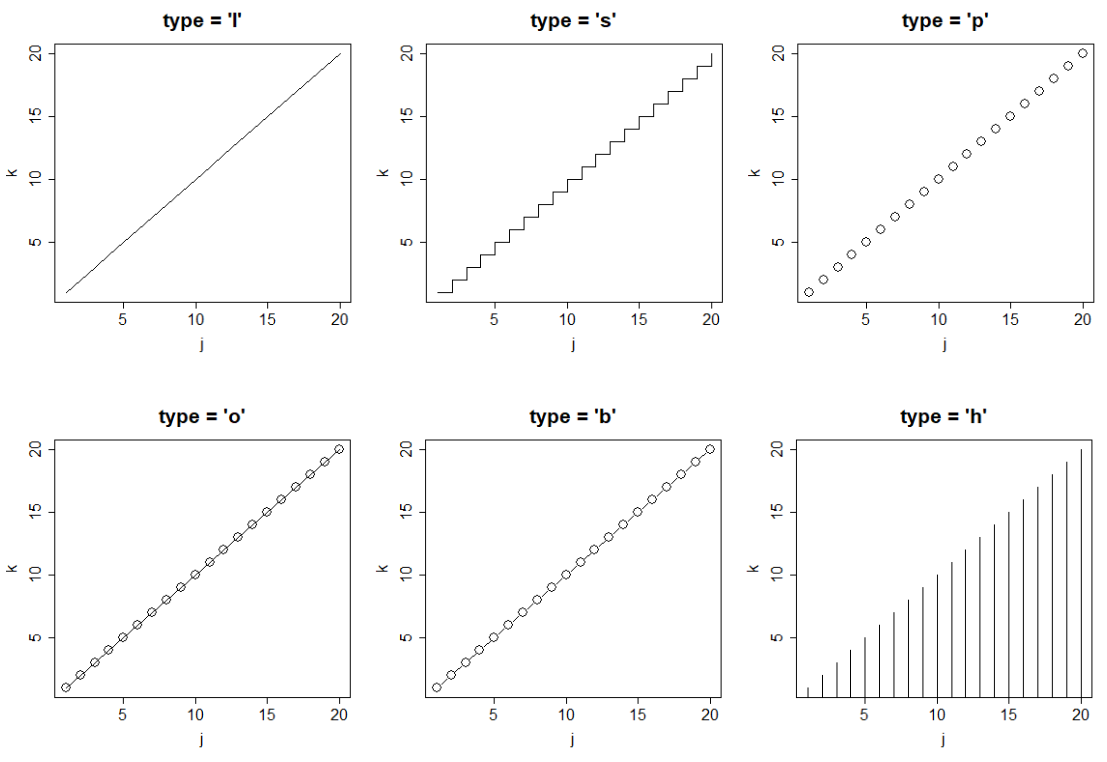
\includegraphics[width=0.8\linewidth]{sections/images/2022-08-18-11-24-35.png}

            \label{}
        \end{figure}
        
        \item \lstinline|pch = | \textbf{p}oint \textbf{ch}aracter, value taken in \lstinline|0:25| for defulat point charaters listed below, or use (vector of) charater to specify, e.g. \lstinline|pch = c('❄')|
        \begin{figure}[H]
            \centering
            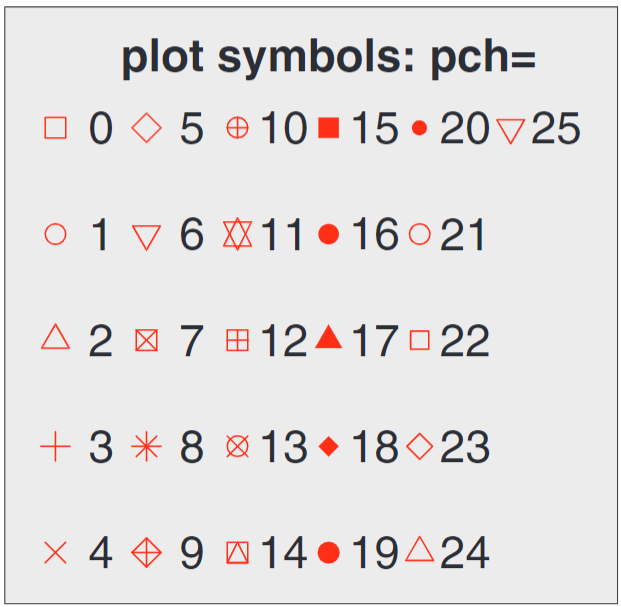
\includegraphics[width=0.3\linewidth]{sections/images/2022-08-18-11-14-15.png}

            \label{}
        \end{figure}

        \item \lstinline|lty = | \textbf{l}ine \textbf{ty}pe, value taken in \lstinline|1:6| (0 for not shown)
        \begin{figure}[H]
            \centering
            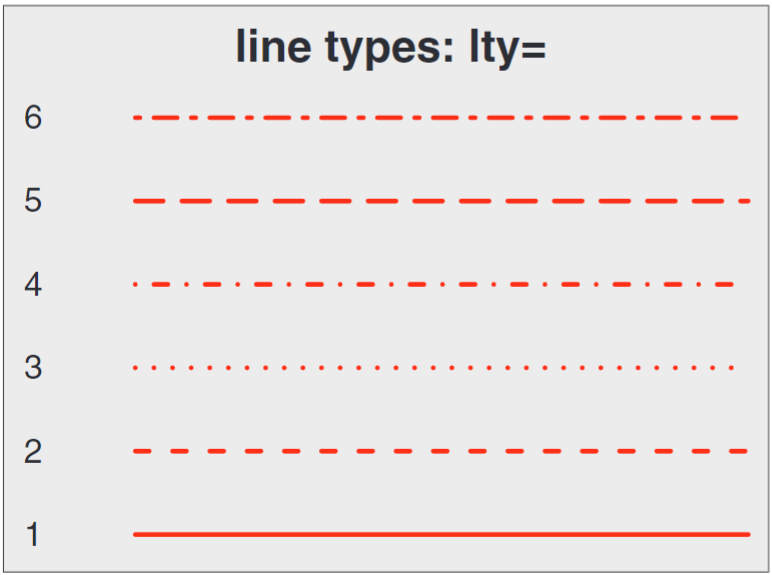
\includegraphics[width=0.4\linewidth]{sections/images/2022-08-18-11-15-34.png}

            \label{}
        \end{figure}

        \item \lstinline|cex = | \textbf{c}haracter \textbf{ex}pansion, relative size with 1 as baseline and default. 
        
        Some derivative function to control size of other plotting elements:
        \begin{itemize}[topsep=2pt,itemsep=0pt]
            \item \lstinline|cex.axis = | relative size of axis node text
            \item \lstinline|cex.lab = | relative size of labels
            \item \lstinline|cex.main = | relative size of title 
            \item \lstinline|cex.sub = | relative size of subtitle 
        \end{itemize}
        
        \item \lstinline|lwd = | \textbf{l}ine \textbf{w}i\textbf{d}th, relative width of line with 1 as baseline and default
        \item \lstinline|col = | \textbf{color} of elements in plot, value examples for color white:
        \begin{itemize}[topsep=2pt,itemsep=0pt]
            \item Index: \lstinline|col = 1| predefined color in \lstinline|R.| 
            \item Color name: \lstinline|col = 'white'|, use \lstinline|colors()| to see all available color names
            \item Hexadecimal code: \lstinline|col = '#FFFFFF'|
            \item RGB code: \lstinline|col = rgb(1,1,1)|, \lstinline|col = rgb(255,255,255, maxColorValue = 255)|
            \item HSV code: \lstinline|col = hsv(0,0,1)|
        \end{itemize}

        \lstinline|col = | can accept vector for various colors, or acccept some function for continuous colors:
        \begin{itemize}[topsep=2pt,itemsep=0pt]
            \item Discrete color: \lstinline|col = c('red','blue')|, or use \lstinline|col = df$GROUP| to color different groups
            \item Continuous color function: \lstinline|rainbow(NUM_OF_COLORS)|, \lstinline|heat_colors()|, \lstinline|terrain.colors()|, \lstinline|topo.colors()|, \lstinline|cm.colors()|
        \end{itemize}

        Some derivative function to control color of other plotting elements:
        \begin{itemize}[topsep=2pt,itemsep=0pt]
            \item \lstinline|col.axis = | color of axis node text
            \item \lstinline|col.lab = | color of labels
            \item \lstinline|col.main = | color of title 
            \item \lstinline|col.sub = | color of subtitle 
            \item \lstinline|bg = | color of background
        \end{itemize}

        \item \lstinline|font = | \textbf{font} used in plot, with 1 = plain, 2 = bold, 3 = italic,
        4 = bold italic

        Some derivative function to control font of other plotting elements:
        \begin{itemize}[topsep=2pt,itemsep=0pt]
            \item \lstinline|font.axis = | font of axis node text
            \item \lstinline|font.lab = | font of labels
            \item \lstinline|font.main = | font of title 
            \item \lstinline|font.sub = | font of subtitle 
            \item \lstinline|ps = | baseline font \textbf{p}oint \textbf{s}ize, i.e. text size = \lstinline|ps*cex|
            \item \lstinline|family = | extra text type, value taken in \lstinline|c('serif', 'sans', 'mono')|m etc. use \lstinline|names(pdfFonts())| to see possible font families
        \end{itemize}
        \item \lstinline|bty = | \textbf{b}ox \textbf{ty}pe of the box surrounding the figure. Value taken in \lstinline|c('o', '7', 'L', 'U', 'C', 'n')| 
    \end{itemize}
    \item \lstinline|axis()| parameters for axis settings: after using \lstinline|xaxt = 'n'| or \lstinline|yaxt = 'n'| to remove correponding axis when executing \lstinline|plot()|, other variation of axis could be made by using \lstinline|axis()|
    \begin{itemize}[topsep=2pt,itemsep=0pt]
        \item \lstinline|axis(1)| for creating $ x $ aixs, \lstinline|axis(2)| for creating $ y $ aixs. Here we would use $ x $ axis in the following parts.
        \item \lstinline|aixs(1, at = )| to specify ticks.
        \item \lstinline|plot(las = )| to specify rotation of ticks, value taken in \lstinline|c('Parallel', 'Horizontal', 'Perpendicular', 'Vertical')|
        \item \lstinline|plot(xlim = c( , ), ylim = c( , ))| for axis limits
        \item \lstinline|plot(log = )| for log transfrom on axis, value taken in \lstinline|c('x', 'y', 'xy')|. 
    \end{itemize}
    
        

    \item \lstinline|legend()| parameters:
    \begin{itemize}[topsep=2pt,itemsep=0pt]
        \item \lstinline|x = | position of legend, value taken in \lstinline|c("top", "bottom", "topleft", "topright", "bottomleft", "bottomright")|
        \item \lstinline|inset = |
        \item other parameters are set following the setting in \lstinline|plot|. An example:
\begin{lstlisting}[language=R]
legend("bottomright", legend = c("red", "green"), lty = c(2,4), lwd = 3, col = c("red", "green"))
\end{lstlisting}

    \end{itemize}

    \item \lstinline|text(X_COOR, Y_COOR, labels = TEXT)| parameters for adding text in figure. An application is \lstinline|text(df$X, df$Y, labels = df$Z)| to label each point.
    \begin{itemize}[topsep=2pt,itemsep=0pt]
        \item \lstinline|pos = | \textbf{pos}ition of text around the coordinate point, value taken in \lstinline|c(1,2,3,4)| 
    \end{itemize}
    
    \item \lstinline|lines()| to put an extra line on existing figure (device). Parameters are similarly set as \lstinline|plot()|
    
    \item \lstinline|par()| to set global \textbf{par}ameters. An example to put 3 different figure in the same device:
\begin{lstlisting}[language=R]
opar <- par(no.readonly = TRUE) # copy original setting
par(mfrow = c(1,3))
plot()
plot()
plot()
par(opar)
\end{lstlisting}

\end{itemize}

\begin{point}
    More Charts
\end{point}

\begin{itemize}[topsep=2pt,itemsep=0pt]
    \item \lstinline|barplot(counts, horiz, besides, ...)| for bar plot. Data should be first prepared by \lstinline|counts <- table(Y_TO_COUNT)|. 
    \item \lstinline|hist(x, breaks, freq, ...)| for histogram.
    \item \lstinline|plot(density(df, kernel = ), ...)| for density plot.
    \item \lstinline|boxplot(x, ...)| for box plot. use \lstinline|boxplot(x ~ GROUP, data = , ...)| to plot grouped boxplot
    \item \lstinline|dotchart(x, labels, groups, ...)| to compare \lstinline|x| value for categories
\end{itemize}


\subsubsection{R::ggplot2 Plotting}
    \lstinline|ggplot2|: \textbf{G}rammar of \textbf{G}raphics \textbf{plot} (2nd edi). It provides a convenient way to produce fancy plots. Reference see \url{https://ggplot2.tidyverse.org/reference/}\index{ggplot2}
    
    Basic steps for \lstinline|ggplot2|:
    \begin{enumerate}[topsep=2pt,itemsep=2pt]
        \item Specify data and arsthetic mapping
        \item Adding 'layers' with \lstinline|geom_|
        \item Adding labels
    \end{enumerate}

    An example:
\begin{lstlisting}[language=R]
ggplot(data=mtcars, aes(x=wt, y=mpg)) +
    geom_point(pch=17, color="blue", size=2) +
    geom_smooth(method="lm", color="red", linetype=2) +
    labs(title="Automobile Data", x="Weight", y="Miles Per Gallon")
\end{lstlisting}


    Elements in \lstinline|ggplot2|:
    \begin{itemize}[topsep=2pt,itemsep=0pt]
        \item \lstinline|aes()| to specify \textbf{aes}thetic mapping, e.g. \lstinline|aes(x = , y = , col = , ...)|. Used in \lstinline|ggplot()| as global setting, in \lstinline|geom_()| as local override (different \lstinline|geom_()| may need different local settings). Examples:
\begin{lstlisting}[language=R]
aes(x = mpg ^ 2, y = wt / cyl, col = am)
#> Aesthetic mapping: 
#> * x -> mpg^2
#> * y -> wt/cyl
#> * color -> am
\end{lstlisting}

        \item \lstinline|geom_| layer to specify statistical figure you want. Some useful plot:
\begin{table}[H]
    \centering
    \renewcommand\arraystretch{1.15}
    \begin{tabularx}{0.9\linewidth}{XXp{0.5\linewidth}}
        \hline
        \hline
        \lstinline|geom_()| Function    &Charts         &Options\\
        \hline
        \lstinline|geom_bar()|          &bar plot       &\lstinline|color, fill, alpha|\\
        \lstinline|geom_boxplot()|      &box plot       &\lstinline|color, fill, alpha, notch, width|\\
        \lstinline|geom_density()|        &density plot   &\lstinline|color, fill, alpha, linetype|\\
        \lstinline|geom_histogram()|    &histogram      &\lstinline|color, fill, alpha, linetype, binwidth|\\
        \lstinline|geom_hline()|        &horizontal line            &\lstinline|color, alpha, linetype, size|\\
        \lstinline|geom_vline()|        &vertical line            &\lstinline|color, alpha, linetype, size|\\
        \lstinline|geom_line()|         &line gragh     &\lstinline|color, alpha, linetypem size|\\
        \lstinline|geom_point()|        &scatter plot       &\lstinline|color, alpha, shape, size|\\
        \lstinline|geom_smooth()|       &fitted line        &\lstinline|method, formula, color, fill, linetype, size|\\
        \lstinline|geom_violin()|       &violin plot        &\lstinline|color, fill, alpha, linetype|\\
        \lstinline|geom_text()|     &text annotation        &see functon help\\
        \hline
        \hline
    \end{tabularx}
\end{table}
        \item \lstinline|labs(title, x, y)| to specify labels and title
        \item \lstinline|facet_grid()| and \lstinline|facet_wrap()| to plot multiple plot, with factor levels as categories, parameters:
        \begin{itemize}[topsep=2pt,itemsep=0pt]
            \item \lstinline|facets = | facet variable. For \lstinline|facet_wrap()| use \lstinline|~VAR1| (one variable); \lstinline|facet_grid()| use \lstinline|.~VAR1| or \lstinline|VAR1~.| or \lstinline|VAR1~VAR2| (allow two variable)
            \item \lstinline|nrow = , ncol = | grid shape
            \item \lstinline|shrink = | whether adjust ticks, set \lstinline|TRUE| or \lstinline|FALSE|
            \item \lstinline|drop = | whether drop levels with censored data, set \lstinline|TRUE| or \lstinline|FALSE|
        \end{itemize}
        \item \lstinline|theme()| to set fonts, backgrouds, gridlines, etc. 
        
        There are some pre-defined theme: \lstinline|theme_grey(), theme_bw(), theme_linedraw(), theme_light(), theme_dark(), theme_minimal(), theme_classic(), theme_void(), theme_test()|.
        
        
        Detailed elements in a plot is adjust by passing \lstinline|element_()|:
        \begin{itemize}[topsep=2pt,itemsep=0pt]
            \item \lstinline|element_line()| set some line element
            \item \lstinline|element_rect()| set some rectangular element
            \item \lstinline|element_text()| set some text element
        \end{itemize}
        
        Some useful command:
        \begin{itemize}[topsep=2pt,itemsep=0pt]
            \item \lstinline|plot.title = element_text(hjust = 0.5)| adjust position of title to mid. Other similar parameters: \lstinline|plot.background, plot.title.position, plot.subtitle, plot.caption, plot.caption.position, plot.tag, plot.tag.position, plot.margin|
            \item \lstinline|panel.background = element_rect(fill = 'white', color = 'blue')| adjust figure background and border. Other similar parameters: \lstinline|panel.grid.major/minor.x/y|
            \item \lstinline|aspect.ratio = | height:width
            \item \lstinline|legend.position = 'none'| to remove automatic legend
        \end{itemize}
        
            
        
            
        
            
        \item \lstinline|ggsave('FILE_NAME', PLOT, WID, HEI)|, or use \lstinline|ggsave('FILE_NAME')| to save the active device.
    \end{itemize}
    
        
    
        



    


